% -*- TeX-master: "../all_the_notes.tex" -*-

\newpage
\section{Flux Qubit 4JJ-linear}
\label{sec:flux-qubit-4jj}

Now lets repeat the same procedure, but with 4 JJs: 3JJ have E$_{J}, C$, while the odd one out
has $\alpha E_J, \alpha C$.

\begin{figure}[h]
  \centering 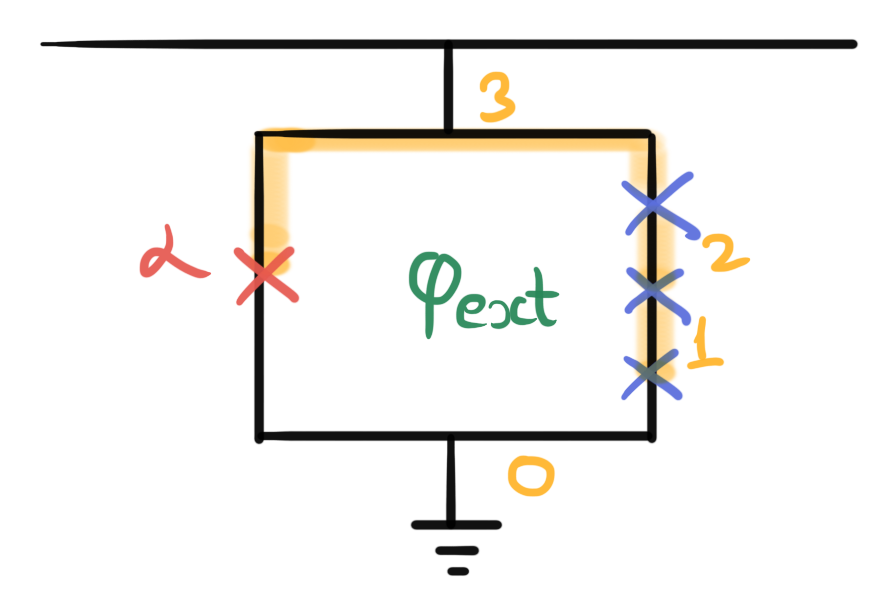
\includegraphics[height=5cm]{flux4jj_linear}
  \caption{\small  One  of  the  junctions  is  scaled   by  a  factor  $\alpha$  relative  to  the
    others \label{fig:flux4jj_linear}}
\end{figure}


\begin{enumerate}
\item Capacitance system reads:
  \begin{equation}
    \label{eq:4jjlinear_1}
    \vec{n} = \frac{C\vec{V}}{2e} \equiv \begin{bmatrix}
      C\left(V_1-0\right) + C\left(V_1-V_2\right) \\
      C\left(V_2-V_1\right) + C\left(V_2-V_3\right) \\
      C\left(V_3-V_2\right) + \alpha C\left(V_3-0\right) \\
    \end{bmatrix} = \iabs{C} \begin{pmatrix}
      2 & -1 & 0\\
      -1 & 2 & -1\\
      0 & -1 & 1 + \alpha
    \end{pmatrix}\begin{pmatrix}
      V_{1}\\V_2\\V_{3}.
    \end{pmatrix}
  \end{equation}

  \noindent
\item The Total Hamiltonian, just like in Ch.~(\ref{eqn:l23JJ}), is
  \begin{equation}
    \label{eq:4jjlinear_2}
    \begin{aligned}
      \mathcal{H} & = \red{U_{\text{kinetic}}} + \blue{U_{\text{potential}}}\\ & =
      \red{\frac{(2e)^2}{2}\vec{n}^{\text{T}}C^{-1}\vec{n}} \\
      &  \qquad +  \blue{\frac{E_J}{2}\bigg[3+\alpha  -  \cos(\varphi_{10}) -  \cos(\varphi_{21})  - \cos(\varphi_{32})  -
        \alpha\cos(\varphi_\text{ext}-\varphi_{10} - \varphi_{20} - \varphi_{30})\bigg]}.
    \end{aligned}
  \end{equation}

  \noindent which can be solved in the number, $ \hat{n} $, of flux, $ \vec{\varphi} $ basis.
\end{enumerate}

\subsection{Number basis}
\label{sec:number-basis}

This was what was done previously. Term by term:

\begin{equation}
  \label{eq:4jjlinear_3}
  \begin{aligned}
    &\red{\frac{(2e)^2}{2}\vec{n}^{\text{T}}C^{-1}\vec{n}}\qquad\qquad E_C \iabs{C} \sum_{n_{1},n_{2},n_3}\iketbra{n_{1},n_2,n_3}{n_{1},n_2,n_3}\vec{n}^TC^{-1}\vec{n}\\
    & \blue{\cos(\varphi_{10}):}\qquad\qquad -\frac{E_J}{2}\bigg[\ketbra{n_1-1}{n_1}+\ketbra{n_1+1}{n_1}\bigg]\otimes \mathbb{I}_{2,}\\
    & \blue{\cos(\varphi_{21}):}\qquad\qquad - \frac{E_J}{2}\bigg[\ketbra{n_1+1}{n_1}\ketbra{n_2-1}{n_2}+\ketbra{n_1-1}{n_1}\ketbra{n_2+1}{n_2}\bigg]\otimes\mathbb{I}_3\\
    & \blue{\alpha\cos(\varphi_\text{ext}-\varphi_{1} - \varphi_{2} - \varphi_{3}):}\qquad\qquad -\frac{E_J}{2}\left(e^{i\varphi_{ext}}e^{-i\varphi_{1}}e^{-i\varphi_2}e^{-i\varphi_{3}} + cc.\right)\\
    &      \qquad       =      -\frac{E_{J}}{2}       e^{i\varphi_{ext}}      \left(\sum_{n_{1},n_{2},n_{3}}
      \iketbra{n_{1}-1,n_{2}-1,n_{3}-1}{n_1,n_2,n_{3}}\right) + cc.
  \end{aligned}
\end{equation}

\noindent Plug this into a matrix and solve. Simple as that.


\subsection{Voltage Dipole Transition}
\label{sec:volt-dipole-trans}

Transition of the system between the ground  and first excited states, will change the voltage
on island 3. The characteristic change is

\begin{equation}
  \label{eq:4jjlinear_3}
  \ibra{e}\hat{V}_3 \iket{g},
\end{equation}

\noindent where $ V_{3} $ is found from Eq.~\ref{eq:4jjlinear_1}:

\begin{equation}
  \label{eq:4jjlinear_4}
  \begin{aligned}
    \vec{V} & = 2eC^{-1}\vec{n} = \frac{2e}{\iabs{C}(1+3\alpha)}\begin{pmatrix}
      1 + 2\alpha & 1 + \alpha & 1 \\
      1 + \alpha & 2 + 2\alpha & 2\\
      1 & 2 & 3
    \end{pmatrix}\\
    &\\
    V_3                     &                      =                     \frac{E_{C}}{\iabs{e}
      (1+3\alpha)}\left[\hat{n}_1+2\hat{n}_{2}+3\hat{n}_{3}\right].
  \end{aligned}

\end{equation}

\noindent
